\documentclass[11pt]{article}

\usepackage{amsmath}
\usepackage{amsfonts}
\usepackage{amssymb}

% Give ourself extra space for text
\usepackage[left = 2.2cm, right = 2.2cm, top = 1.8cm, bottom = 2.8cm]{geometry}

% Allows us to easily change the numbering system used in things like \begin{enumerate}. https://ctan.org/tex-archive/macros/latex/contrib/enumitem/
\usepackage[shortlabels]{enumitem}

% Turns table of contents, \refs, etc. into hyperlinks
\usepackage{hyperref}

% To include image, just use \includegraphics[scale=•]{relative path to image}
\usepackage{graphicx}
\graphicspath{ {./images/} }

% Common sets
\newcommand{\integers}{\mathbb{Z}}
\newcommand{\naturals}{\mathbb{N}}
\newcommand{\reals}{\mathbb{R}}

% Power set
\newcommand{\powerset}{\mathcal{P}}

% Identity matrix
\newcommand{\ident}{\mathbb{I}}

% Inverse hyperbolic functions
\DeclareMathOperator{\arcosh}{arcosh}
\DeclareMathOperator{\arsinh}{arsinh}
\DeclareMathOperator{\artanh}{artanh}

% I hat, J hat, K hat
\newcommand{\ihat}{\boldsymbol{\hat{\textbf{\i}}}}
\newcommand{\jhat}{\boldsymbol{\hat{\textbf{\j}}}}
\newcommand{\khat}{\boldsymbol{\hat{\textbf{k}}}}

% Better vectors (for single characters)
\renewcommand{\vec}[1]{\mathbf{#1}}

% Allows us to number equations in \begin{align} statements, etc.
\newcommand\numberthis{\addtocounter{equation}{1}\tag{\theequation}}

% Augmented matrices: this allows us to make augmented matrics using something like \begin{bmatrix}[cc|c]. Taken from Stefan Kottwitz at https://tex.stackexchange.com/questions/2233/whats-the-best-way-make-an-augmented-coefficient-matrix.
\makeatletter
\renewcommand*\env@matrix[1][*\c@MaxMatrixCols c]{%
  \hskip -\arraycolsep
  \let\@ifnextchar\new@ifnextchar
  \array{#1}}
\makeatother

% NOTE: This means \section does NOT number sections, but ensures that they appear in the table of contents, which does not occur if simply \section* is used. From egreg @ https://tex.stackexchange.com/a/30225.
\setcounter{secnumdepth}{0} % sections are level 1

\begin{document}
\title{ENG1005: Lecture 26}
\author{Lex Gallon}
\maketitle

\tableofcontents

\section*{Video link}
\url{https://echo360.org.au/lesson/G_32340f5d-ff38-43d2-be9d-d88ddb1b3611_b944cecf-8ba5-40d3-a870-0243a0a9e78c_2020-05-20T14:58:00.000_2020-05-20T15:53:00.000/classroom#sortDirection=desc}

\subsection{Examples - continued}
\begin{enumerate}[ (i) ]
\setcounter{enumi}{2}
\item $f(x, y) = y^2 - x^2$.
\begin{align*}
\nabla f(x, y) &= (-2x, 2y) \\
\nabla f(0, 0) &= (0, 0) \Rightarrow (0, 0) \text{ is a critical point }
\end{align*}
But note that it is neither a maximum or a minimum. It is a \textbf{saddle point}.

\begin{center}
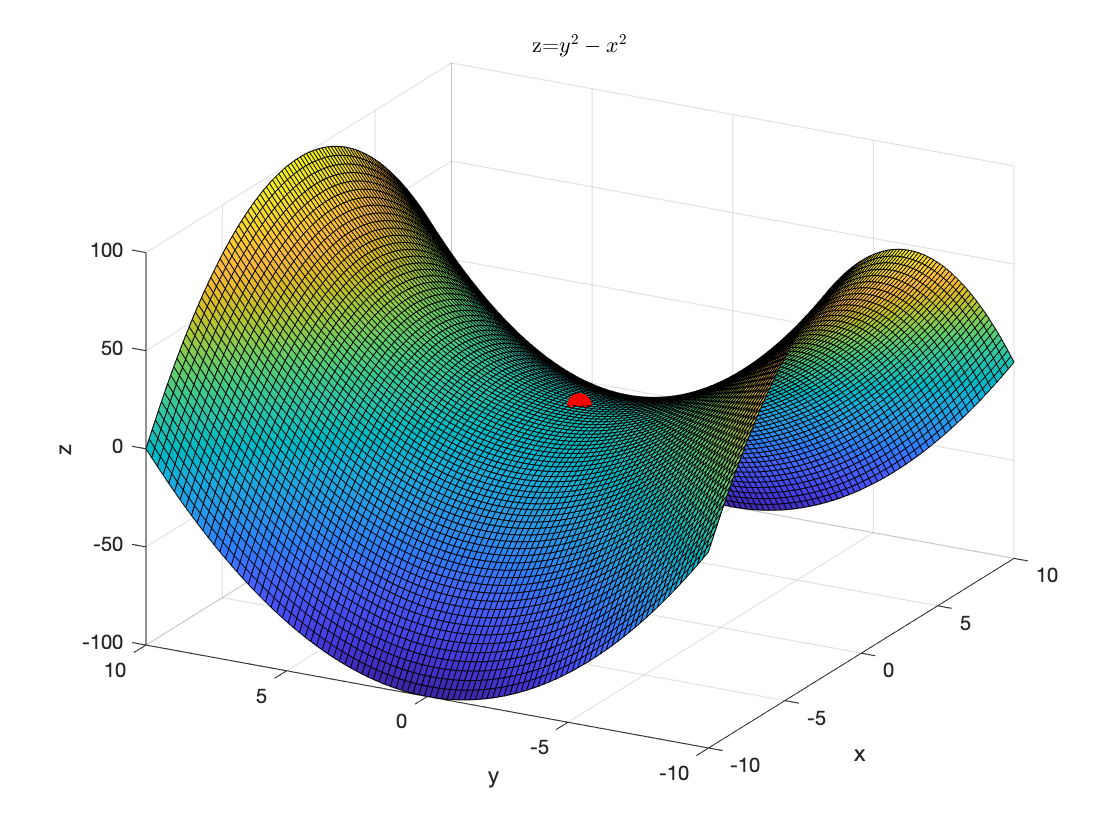
\includegraphics[scale=0.25]{eg3}
\end{center}

\item $f(x, y) = \sqrt{x^2 + y^2}$
\begin{align*}
\nabla f(x, y) &= (\frac{2x}{\sqrt{x^2 + y^2}}, \frac{2y}{\sqrt{x^2 + y^2}}) \\
\nabla f(0, 0) \text{ DNE }
\end{align*}
This is still a critical point, and from the graph it is clear that this is an absolute minimum.

\begin{center}
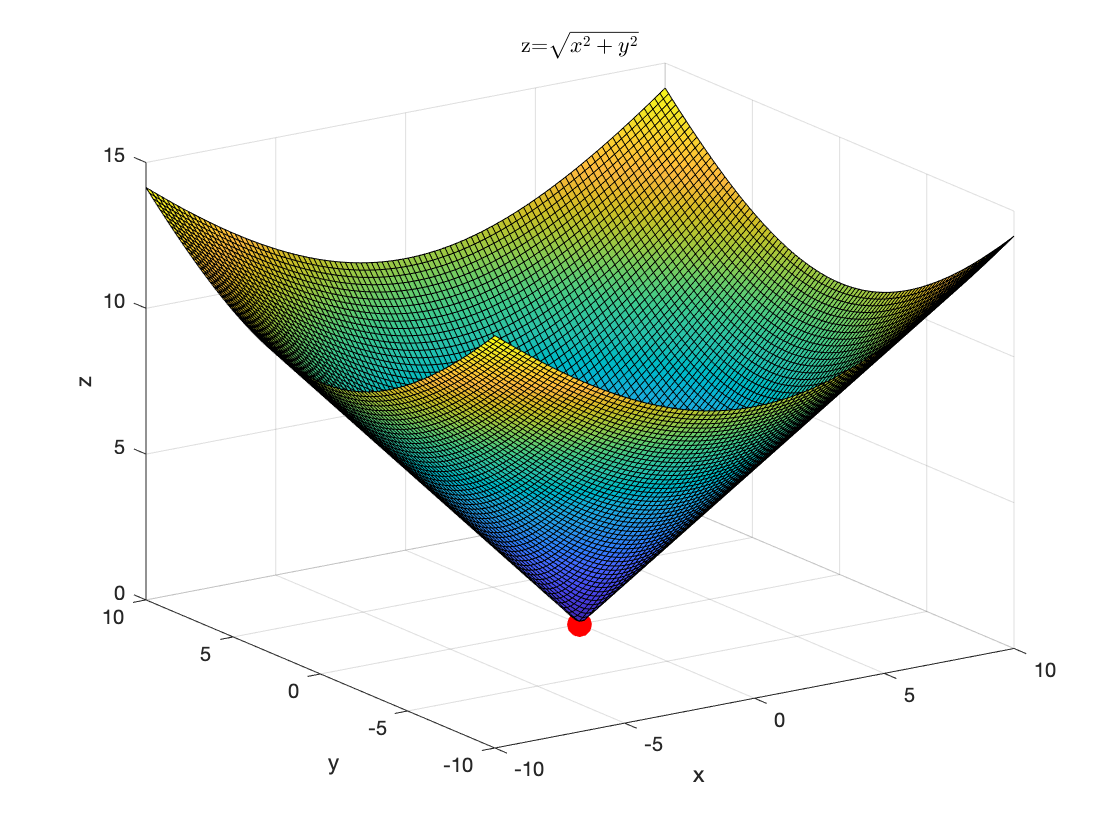
\includegraphics[scale=0.25]{eg4}
\end{center}

\end{enumerate}

\subsection{Example}
Let $f(x, y) = 4xy - x^ - y^4$. Find all the critical points of $f(x, y)$. 

\subsection{Solution}
\begin{align*}
\nabla f(x, y) = \vec{0} &\Rightarrow \left\{ \begin{array}{c}
\frac{\partial f}{\partial x} = 4y - 4x^3 = 0 \\
\frac{\partial f}{\partial x} = 4x - 4y^3 = 0 \\
\end{array} \right. \\
&\Rightarrow \left\{ \begin{array}{c}
y = x^3 \\
x - y^3 = 0 \\
\end{array} \right. \\
&\Rightarrow x - x^9 = 0 \\
&\Rightarrow x(x - x^8) = 0
&\Rightarrow x = 0 \text{ or } x^8 = 1 \\
&\Rightarrow x=0, \pm 1
\end{align*}

Therefore,
\[ (0, 0), (1, 1), (-1, -1) \]
are all the critical points of $f(x, y)$.

\section{Classifying critical points §9.7.2}
\subsection{Theorem}
Suppose $f(x, y)$ and its derivatives up to 3rd order are continuous on $B_R((a, b))$, $\nabla f(x, y) = \vec{0}$ and let
\[ A = \frac{\partial^2 f}{\partial x^2}(a, b),\ B = \frac{\partial^2 f}{\partial x \partial y}(a, b) \text{ and } C = \frac{\partial^2 f}{\partial y^2}(a, b) \]
then
\begin{enumerate}[ (i) ]
\item $f(x, y)$ has a local minimum at $(a, b)$ if $AC > B^2$ and $A > 0$.
\item $f(x, y)$ has a local maximum at $(a, b)$ if $AC > B^2$ and $A < 0$.
\item $f(x, y)$ has a saddle point at $(a, b)$ if $AC < B^2$.
\item and the test gives no information if $AC = B^2$.
\end{enumerate}

\subsection{Example}
Classify all the critical points of $f(x, y) = 4xy - x^4 - y^4$.

\subsection{Solution}
From before, we know that the critical points are
\[ (0, 0), (1, 1), (-1, -1) \]
Now,
\begin{align*}
\frac{\partial^2 f}{\partial x^2} &= -12 x^2 &\left( A = \frac{\partial^2 f}{\partial x^2}(a, b) \right) \\
\frac{\partial^2 f}{\partial y^2} &= -12 y^2 &\left( C = \frac{\partial^2 f}{\partial y^2}(a, b) \right) \\
\frac{\partial^2 f}{\partial x \partial y} &= 4 &\left( B = \frac{\partial^2 f}{\partial x \partial y}(a, b) \right)
\end{align*}

and 
\[ \frac{\partial^2 f}{\partial x^2} \frac{\partial^2 f}{\partial y^2} - \left( \frac{\partial^2 f}{\partial x \partial y} \right)^2 = 144x^2y^2 - 16 \quad \left(AC - B^2\right) \]

\begin{tabular}{c|c|c|c}
Critical point & $A$ & $AC - B^2$ & Conclusion \\
\hline
$(0, 0)$ & 0 & $-16 < 0$ & Saddle point\\
$(1, 1)$ & $-12 < 0$ & $128 > 0$ & Local max\\
$(-1, -1)$ & $-12 < 0$ & $128 > 0$ & Local max \\
\end{tabular}

\section{Absolute maxima and minima §9.7.4}
\subsection{Theorem}
If $D \subset \reals^2$ is closed and bounded and $f(x, y)$ is continuous on $D$ then there exists points in $D$ where $f(x, y)$ achieves an absolute maximum and an absolute minimum.

\subsection{Terminology}
\begin{itemize}
\item $D$ is bounded if $D \subset B_R(\vec{0})$ for some $R > 0$.
\item $D$ is closed if it is defined by closed inequalities.\\
e.g. \begin{align*}
D &= \{ (x, y) | x^2 + y^2 \leq 1 \text{ and } x + y \geq 1 \} \text{ is closed}. \\
D &= \{ (x, y) | x^2 + y^2 \leq 1 \text{ and } x > 0 \} \text{ is NOT closed}.
\end{align*}
Note the $\geq$ as opposed to the $>$. I'll have to check but I believe what Todd means is that it is closed if there is an equality, not simply a $>$ or $<$.
\end{itemize}

\end{document}